%
% File: chap01.tex
% Author: Andreas Selinger
%
\let\textcircled=\pgftextcircled
\chapter{Matrix Multiplications}
\label{chap:matmult}


%=======
%\section{Intro}
\initial{T}he multiplication of two matrices is an essential part of linear algebra and it is of vital importance for all of modern physics and modelling. It is used for example for the numerical solution of linear systems and eigenvalue problems or, on a lower level, for transforming a matrix from one vector space to another.

The matrix multiplication is defined as follows: Given an $m\times r$ matrix $G$ and an $r \times n$ matrix $H$, a matrix element of their product $P$ is defined as 
\begin{align}
p_{i,j} = g_{i,1} h_{1,j} + g_{i,2} h_{2,j} + \hdots + g_{i,r} h_{r,j} = \sum_{k} g_{i,k} h_{kj}  ,
\end{align}
with matrix elements
\begin{align}
\label{equ:def_matmatmult}
GH = \begin{bmatrix}
           & \vdots &  &   \\    
    g_{i,1} & g_{i,2} & \hdots & g_{i,r} \\
       & \vdots &  &   \\    
\end{bmatrix}
\begin{bmatrix}
           & h_{1,j} &  &   \\    
  \hdots   & h_{2,j} & \hdots & \\
    & \vdots & \\
       & h_{3,j} &  &   \\    
\end{bmatrix} = 
\begin{bmatrix}
           & \vdots &  &   \\    
    \hdots & p_{i,j} & \hdots \\
       & \vdots &  &   \\    
\end{bmatrix}
\end{align}
This means that the $(i,j)$-\textit{th} entry of the product is the dot product of the $i$-th row of the left matrix with the $j$-th column of the right matrix~\cite{hefferon2012linear}. 

There are very simple ways to store matrices on a computer, e.g. the elements of an $m\times n$ matrix can be stored row per row in an array of length $m\cdot n$. Accessing the elements is also very simple then: element $a_{i,j}$ corresponds to the $(i\cdot n + j)$-th entry of the array (zero based numbering for the array and the matrix provided). However, storing matrices in such a dense format is very often not suitable, as described in the next section. 

\section{Storing Sparse Matrices}
There are many applications, where only a small percentage of the elements of a matrix are non-zero, for example the matrices that arise from the discretization of partial differential equations. Storing them as dense matrices would be infeasible and very often not possible, because there might not be enough memory and also, algorithms for dense matrices would take vast amounts of time. Therefore, different data structures and algorithms have to be designed for such sparse matrices. 

There are formats for sparse matrices with a special structure, for example for banded or for diagonal symmetric matrices. For general sparse matrices, some of the formats are:

\begin{itemize}
\item List of lists: For this method of storing matrices, there is a list for each row of the matrix. Each entry of the list contains the column index and the value \cite{python}.
\item Coordinate list: In coordinate lists, matrix elements are stored in a list of (row, column, value) tuples. In order to improve random access times, these entries should be sorted by row and column indices \cite{python}.
\item Dictionary of keys: Here the (row, column)-pairs map to the values of the matrix. If there is no key for a certain matrix entry, this entry is assumed to be zero. This format is an efficient structure if the matrix is constructed incrementally \cite{python}.
\item Compressed sparse row (CSR, also called AIJ-format): In the CSR-format, there are three arrays: One for the size of each row, one for the column indices and one for the non-zero values of the matrix.
\item Compressed sparse column (CSC): This is basically the transposed CSR-format, so instead of rows, columns are stored here. 
\end{itemize}

Of the formats mentioned, CSR and CSC are best suited for high performance computing. The other formats might be quicker or simpler to construct, but the access to these matrices might lack in performance. As CSR is the format that is used in the work connected to this thesis, it will be discussed in more detail in the following section.

\subsection{CSR format}
\label{sec:csr_format}
The compressed sparse row format is the default format for sparse parallel matrices in the parallel computing library PETSc \cite{petsc-web-page}. It uses three one-dimensional arrays \texttt{Aa}, \texttt{Aj} and \texttt{Ai} to store a matrix \texttt{A}. These arrays are explained with the following $6 \times 6$ example matrix:
\begin{align}
\texttt{A} = 
\begin{bmatrix}
& 0 & 0 & \color{red}{-3} & 0  & 0  & 0  \\
                           & 0 & 0 & 0  & 0  & 0  & \color{red}{8}  \\
 & 0 & 0 & 0  & 0  & \color{red}{9}  & 0  \\
                           & \color{red}{5} & \color{red}{2} & \color{red}{10} & \color{red}{-1} & 0  & 0  \\
 & 0 & 0 & 0  & 0  & 0  & \color{red}{6}  \\
                           & \color{red}{4} & 0 & 0  & \color{red}{-2} & \color{red}{-4} & \color{red}{-5}
\end{bmatrix}
\label{equ:csr_example}
\end{align}

\begin{itemize}
\item \texttt{Aj} gives the column indices of the non-zero values, row per row. Hence, its length is the number of non-zero elements. For the example matrix \texttt{A}, \texttt{Aj = [2, 5, 4, 0, 1, 2, 3, 5, 0, 3, 4, 5]}
\item \texttt{Aa} gives the non-zero values of the matrix, so its length is the number of non-zero elements as well. In the example, \texttt{Aa = [-3, 8, 9, 5, 2, 10, -1, 6, 4, 0, 0, -2, -4, -5]}.
\item \texttt{Ai} is used to store the sizes of the rows. In this array of size $n+1$ (with the number of rows in the matrix = $n$), the element with the index 0 is  always 0. After that, the $i$-th element tells how many non-zero elements are encountered when going through the matrix from the first row to the (included) $i$-th row. Therefore, the  \texttt{Ai} array is \texttt{Ai = [0, 1, 2, 3, 7, 8, 12]}.
\end{itemize}

\subsection{Multi-Process Matrices}
In PETSc, matrices can be sequential matrices or parallel (MPI) matrices, which means that they are either maintained by one or several processes. The example matrix \texttt{A} from before can be split between three processes as it is shown in Table~\ref{table:div_ex_matrix}.
\begin{table*}[bp]
\centering
\begin{tabular}{ccc|cc|cc}   
% \begin{align}
% \begin{bmatrix}
\multirow{2}{*}{Process 1} & 0 & 0  & \color{red}{-3} & 0  & 0  & 0  \\
                           & 0 & 0  & 0  & 0  & 0  & \color{red}{8}  \\ \hline
\multirow{2}{*}{Process 2} & 0 & 0  & 0  & 0  & \color{red}{9}  & 0  \\
                           & \color{red}{5} & \color{red}{2}  & \color{red}{10} & \color{red}{-1} & 0  & 0  \\ \hline
\multirow{2}{*}{Process 3} & 0 & 0 & 0  & 0  & 0  & \color{red}{6}  \\
                           & \color{red}{4} & 0 & 0  & \color{red}{-2} & \color{red}{-4} & \color{red}{-5}
\end{tabular}
\caption{Splitting the example matrix \texttt{A} (\ref{equ:csr_example}) for three different processes.}
\label{table:div_ex_matrix}
\end{table*}

For some operations, like matrix additions or matrix vector products, it is possible to perform computations that only use the part of the matrix that is local to the respective process. However, there are algorithms, e.g. the matrix-matrix multiplication, that also need access to parts of the matrix which are not local. Hence, lots of data has to be transferred over the network.

PETSc stores the diagonal and off-diagonal entries  of parallel (MPI) matrices separately. That way, specialized algorithms can exploit the fact that there are usually far more diagonal than off-diagonal entries.  In the example from Tab.~\ref{table:div_ex_matrix}, the matrices
\begin{align}
\begin{bmatrix}
0 & 0\\
0 & 0\\
\end{bmatrix},
\begin{bmatrix}
0 & 0\\
10 & -1\\
\end{bmatrix}, \textnormal{ and }
\begin{bmatrix}
0 & 6\\
-4 & -5\\
\end{bmatrix}
\label{mat:diag_example}
\end{align}
are diagonal matrices, and 
\begin{align}
\begin{bmatrix}
-3 & 0 & 0 & 0\\
0 & 0 & 0 & 8\\
\end{bmatrix},
\begin{bmatrix}
0 & 0 & 9 & 0\\
5 & 2 & 0 & 0\\
\end{bmatrix}, \textnormal{ and }
\begin{bmatrix}
0 & 0 & 0 & 0\\
4 & 0 & 0 & -2\\
\end{bmatrix}
\label{mat:diag_example}
\end{align}

are off-diagonal matrices, each of them local to their respective process and each of them starting with the local column index 0. This means that the global column index might be different than the local one, so this global index might have to be computed when the matrix is accessed.

In order to set up parallel matrices quickly, preallocation of memory is crucial. For that, the number of non-zero entries in the diagonal and off-diagonal parts of each row has to be known (or at least an approximate minimum value should be known). Then, the memory for each row can be preallocated and does not have to be extended during the computation, which would be much more expensive than the preallocation \cite{petsc-web-page}.



\section{Introduction to Sparse Matrix-Matrix Multiplication}
A function that is very important for the applications described in this work, is the Sparse Matrix-Matrix Multiplication (SpGEMM)\footnote{The name SpGEMM is derived from BLAS routines, which include DGEMM for double precision general matrix-matrix multiplication, DSYMM for double precision symmetric matrix multiplication, ZHEMM for complex hermitian matrix multiplication, etc.} $C = A B$, with sparse matrices $A, B$ and $C$. In Chapter ~2, this product was used to compute coarse grid operators $L_H$ by multiplying the fine grid operator $L_h$ with restriction interpolation operators: $L_H = I_h^HL_h I_H^h$.
However, compared to the dense GEMM, SpGEMM usually suffers from very poor FLOP performance on parallel hardware. This is due to various reasons:  
\begin{itemize}
\item Irregular memory access patterns: Depending on the structure of the matrices, there are computation steps where not all rows or elements of rows of a matrix are needed, so they are just skipped, which lowers the hit rate of the cache.
\item Load imbalances: Matrices that are obtained from graphs of social networks or from a recommendation system domain often have very dense parts, while other parts of the matrices are sparse. This leads to imbalanced loads among the ranks, so many ranks are idle while only some are still working.
\item Poor data locality: For each off-diagonal element of the matrix $A$, non-local rows have to be requested. This leads to a high amount of traffic over the network, which causes the performance to suffer both due to low bandwidth and high latencies. Fortunately, many non-zero elements in various real life matrices reside in the diagonal portion of a matrix, so relatively few non-local rows have to be requested.  
\item Unknown non-zero structure of the output matrix: In contrast to dense matrix-matrix multiplication, where each element of the output matrix has to be computed, only the non-zero elements have to be computed  for sparse matrix-matrix multiplication. However, this means that the multiplication needs another (work-intensive) step; the computation of the positions of the non-zero elements \cite{intel_algorithm}.
\end{itemize}

\section{Mechanics of Matrix Multiplication}

There are different points of view for matrix multiplication. For example, one can see each result entry as the dot product of row and column vectors, as it was defined earlier in this chapter and as it can be seen in Fig.~\ref{fig:matmult_dot_product}.
\begin{figure}[tb]
\centering
 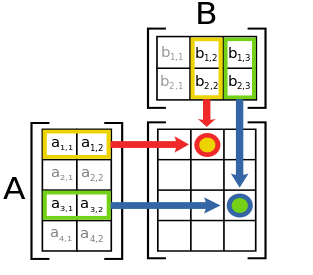
\includegraphics[height=6cm]{matrix_multiplication_wiki}
    %By File:Matrix multiplication diagram.svg:User:BilouSee below. - This file was derived from: Matrix multiplication diagram.svg, CC BY-SA 3.0, https://commons.wikimedia.org/w/index.php?curid=15175268
\caption{Each element of the product of two matrices $\textit{AB} = \textit{C}$ can be seen as the dot product of a row and a column vector: Element $c_{i,j}$ is the dot product of the $i$-th row vector of \textit{A} with the $j$-th column vector of \textit{B}. Figure from the Wikimedia foundation	 \cite{wiki:matrix_multiplication_image}.}
\label{fig:matmult_dot_product}
\end{figure}
However, due to very irregular memory access patterns and low data locality, directly computing dot products of row and column vectors is not the most favourable method for high performance. 



\begin{figure}[tb]
\centering
{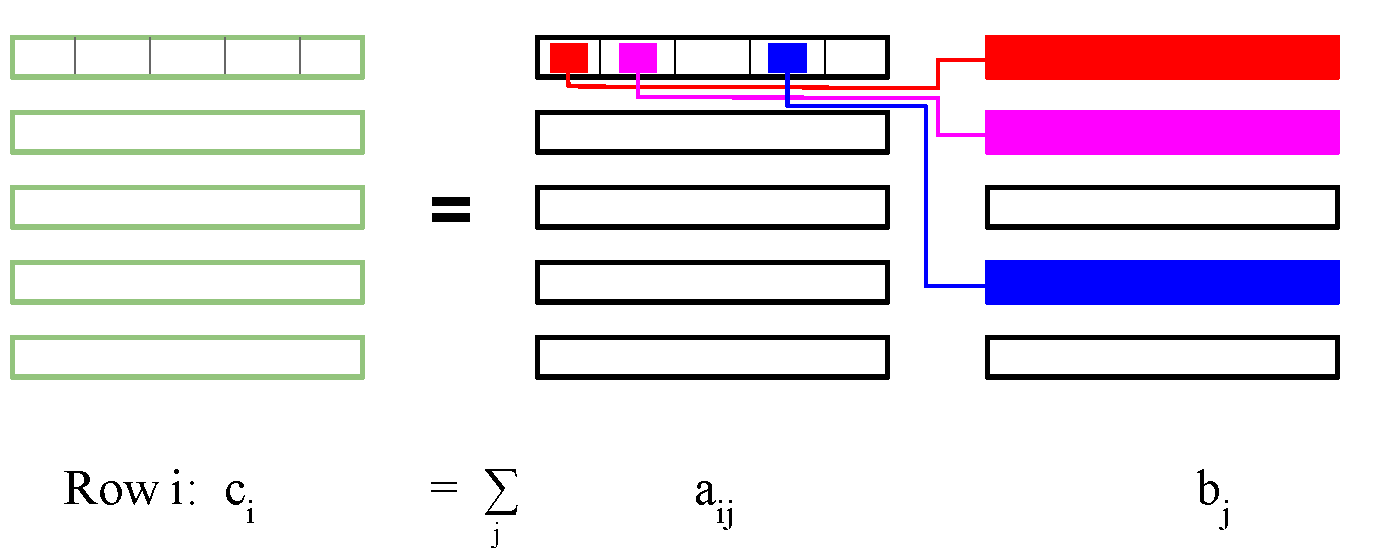
\includegraphics[width=0.9\textwidth]{matrix_multiplication}}
\caption{In order to obtain the first row of $C$, the first row of $B$ is scaled with the first element of the first row of $A$, the second row is scaled with the second element and the fourth row is scaled with the fourth element in the first row of $A$. Then these scaled rows of $B$ are added to form the result $c_1$.}
\label{fig:matmult_petsc}
\end{figure}

The most efficient way to compute the sparse matrix product, is to see it as a weighted summation of rows of \textit{B}. Therefore, this approach is implemented in PETSc. Here, a whole row of \textit{C} is calculated at once. Fig.~\ref{fig:matmult_petsc} shows an illustration of how this multiplication $\textit{C} = \textit{AB}$ works in PETSc. In order to calculate a row in $\textit{C}$, weighted rows of $B$ are added to each other. More precisely; a row $b_j$ is weighted with a factor $a_{ij}$, before it is added to the other rows of $B$ to form a row $c_i$. If an element $a_{ij}$ of a row $a_i$ is zero, a whole row $b_j$ can be skipped. 

In the example of Fig.~\ref{fig:matmult_petsc} this means that the first row of \textit{C} is computed by adding three rows (vectors) to each other: the first row of $B$ scaled with the first element of $a_1$, the second row of $\textit{B}$ scaled with the second element of $a_1$, and the fourth row of $B$ scaled with the fourth element of $a_1$.


As mentioned before, a difference to dense matrix-matrix multiplication is that for the sparse multiplication, also the positions of non-zero entries have to be computed. This part actually takes a large portion of the total amount of time spent on the matrix multiplication. So there are two phases, first a symbolic phase where the positions of the non-zero entries are computed, and then a numeric phase where the numerical values are computed. Now we take a look at these two phases.



\section{Symbolic Phase of the Sequential Algorithm}
There are a few different, already existing implementations for the sequential (single core) version of sparse matrix-matrix multiplication in PETSc. For each row $c_i$ of \textit{C}, the rows $b_j$ that correspond to the non-zero elements $a_{ij}$ have to be merged, i.e. one has to find out which indices of the result row $c_i$ are non-zero. For this process, there are various implementations in PETSc, and they will be discussed in the following.


\subsection{Sorted MatMatMult}
One of the implementations that merge the rows of $B$ for finding out where the non-zeros of the result are, is the \textit{sorted} algorithm. The steps of this algorithm can be seen in Fig.~\ref{fig:spgemm-sorted_1} and Fig.~\ref{fig:spgemm-sorted_2}.

\begin{enumerate}[label=\alph*)]
\item The rows $b_j$ can be seen  with a dashed green frame. Also, there is a dense flag array that is initialized with zeros and indicates which indices of the result row $c_j$ (in red) contain non-zeros. Therefore, the length of this array is the same as the number of columns in the matrix, no matter how many non-zeros there are per row. A segmented buffer (in black) will be used once the calculation starts. 
\item The calculation starts by progressing through the entries of the first row. The first entry of the first row (in brown) is non-zero, so the first element in the dense array is set to 1 and the  column index of this entry (1) is appended to the buffer.
\item In the first row of $B$, there are also non-zero entries at the indices 3 and 6. Since both of the corresponding values in the dense array were 0, they are now set to 1 and the indices are appended to the buffer.
\item In the second row of $B$, there is is non-zero entry at index 3. However, the corresponding value in the dense array is already set to 1, so the index is not appended to the buffer. The index 5 is appended, though.
\item Both indices corresponding to non-zero entries of the third row of $B$ are appended to the buffer.
\item After all rows $b_j$ are processed, the buffer array has to be sorted. This yields the result column indices, so the buffer is copied to the result row of $C$.
\end{enumerate}

\begin{figure}[H]
\centering
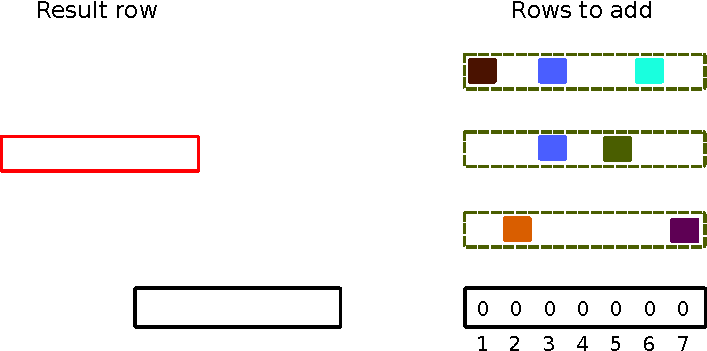
\includegraphics[width=0.72\textwidth]{sorted/spgemm-sorted-3}\\
a)\\
\vspace*{5mm}
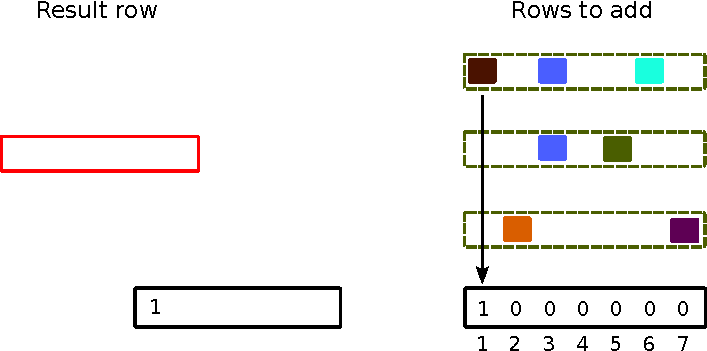
\includegraphics[width=0.72\textwidth]{sorted/spgemm-sorted-4}\\
b)\\
\vspace*{5mm}
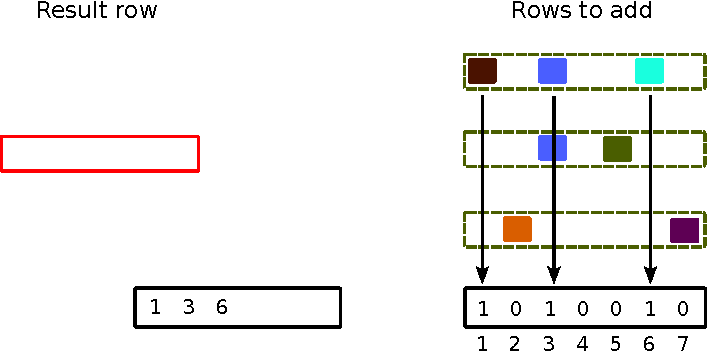
\includegraphics[width=0.72\textwidth]{sorted/spgemm-sorted-6}\\
c)\\
\vspace*{5mm}
\caption{Symbolic matrix-matrix multiplication with the \textit{sorted} algorithm, part 1. Figures by Karl Rupp \cite{karli_LANS_image}.}
\label{fig:spgemm-sorted_1}
\end{figure}

\begin{figure}[H]
\centering
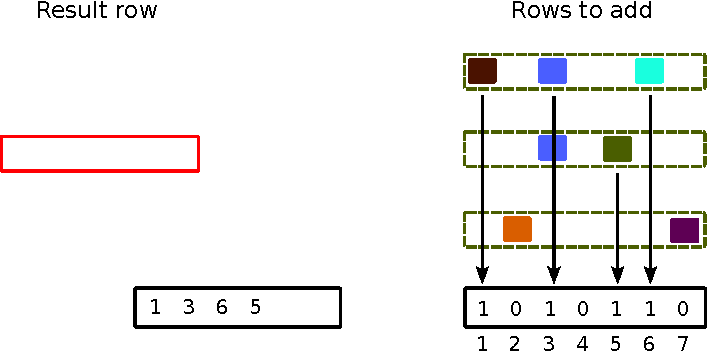
\includegraphics[width=0.72\textwidth]{sorted/spgemm-sorted-7}\\
d)\\
\vspace*{5mm}
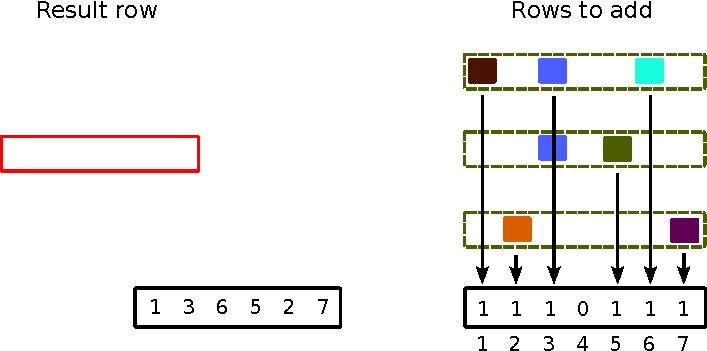
\includegraphics[width=0.72\textwidth]{sorted/spgemm-sorted-9}\\
e)\\
\vspace*{5mm}
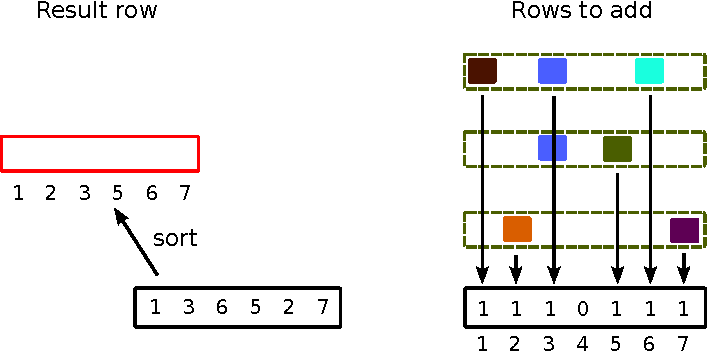
\includegraphics[width=0.72\textwidth]{sorted/spgemm-sorted-10}\\
f)\\
\vspace*{5mm}
\caption{Symbolic matrix-matrix multiplication with the \textit{sorted} algorithm, part 2. Figures by Karl Rupp \cite{karli_LANS_image}.}
\label{fig:spgemm-sorted_2}
\end{figure}


\subsection{Scalable MatMatMult}
The implementation of the \textit{scalable} matrix-matrix multiplication does not need a dense array with a length that only depends on the number of columns. Instead, there is a dynamic data structure, such as a linked list, a heap or some other binary tree that stores only the indices of non-zero entries. For that reason, the memory requirements are much lower than for the \textit{sorted} implementation and these requirements scale with the number of non-zeros. If the non-scalable implementation is used with, for example, a matrix $B$ that has one billion columns and 32-bit integer values are used, this means that 4~GB of data are needed on each MPI-rank just for the dense array. On the other hand, only non-zero indices are stored in the scalable implementation.

In Fig.~\ref{fig:spgemm-scalable_1} and Fig.~\ref{fig:spgemm-scalable_2}, this algorithm is illustrated with the example of a sorted linked list. The steps of the algorithm are:

\begin{enumerate}[label=\alph*)]
\item The rows $b_j$ are shown in green with a dashed frame again. Starting in the first row, the index 1 of the first element is added to a linked list. 
\item Next, the index 3 is added to this linked list.
\item The same is done with index 6. 
\item In the second row, the algorithm first tries to add index 3, but since it already is in the list, it is rejected. So the next index that is added is 5. 
\item In the third row of $B$, the indices 2 and 7 are added to the sorted linked list.
\item After all rows have been processed, the linked list can be copied to the result row array.
\end{enumerate}


\begin{figure}[H]
\centering
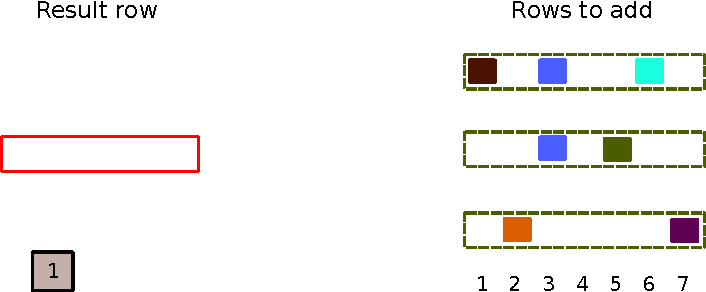
\includegraphics[width=0.72\textwidth]{scalable/spgemm-scalable-3}\\
a)\\
\vspace*{5mm}
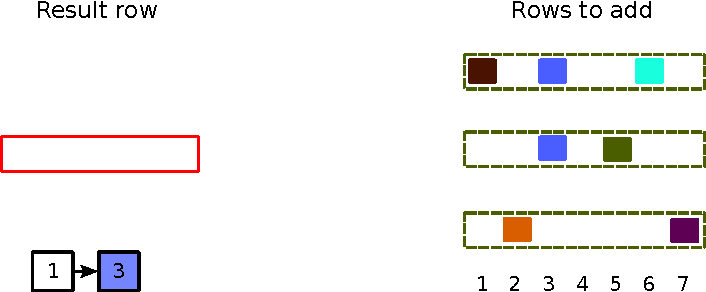
\includegraphics[width=0.72\textwidth]{scalable/spgemm-scalable-4}\\
b)\\
\vspace*{5mm}
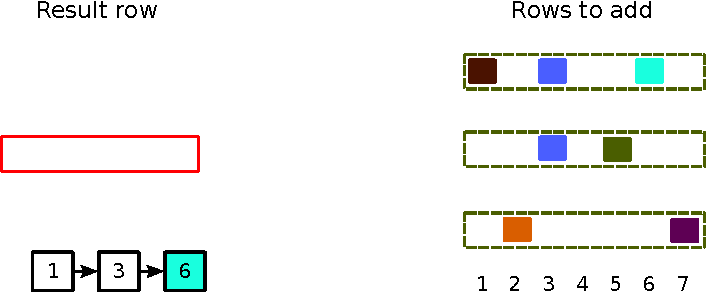
\includegraphics[width=0.72\textwidth]{scalable/spgemm-scalable-5}\\
c)\\
\vspace*{5mm}
\caption{Symbolic matrix-matrix multiplication with the \textit{scalable} algorithm, part 1. Figures by Karl Rupp \cite{karli_LANS_image}.}
\label{fig:spgemm-scalable_1}
\end{figure}


\begin{figure}[H]
\centering
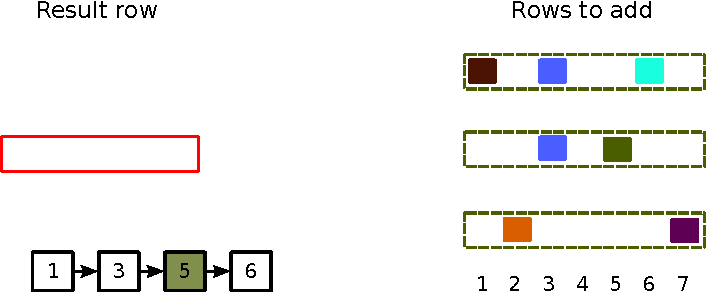
\includegraphics[width=0.72\textwidth]{scalable/spgemm-scalable-6}\\
d)\\
\vspace*{15mm}
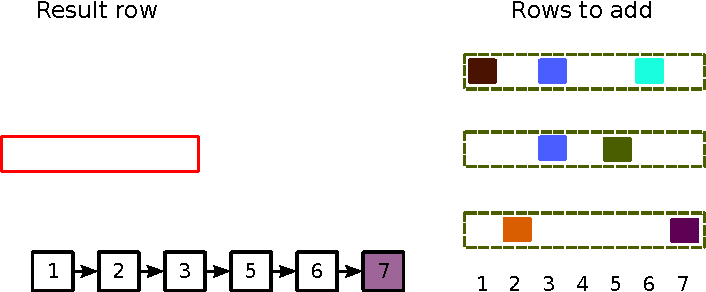
\includegraphics[width=0.72\textwidth]{scalable/spgemm-scalable-8}\\
e)\\
\vspace*{15mm}
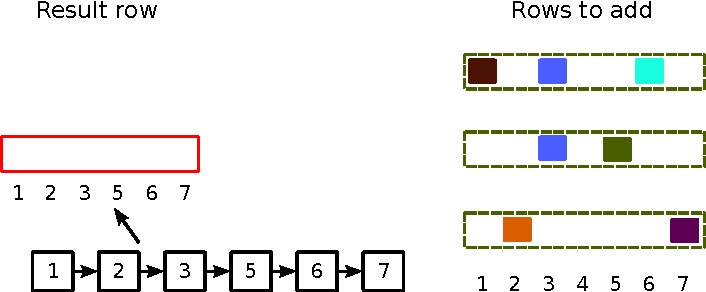
\includegraphics[width=0.72\textwidth]{scalable/spgemm-scalable-10}\\
f)\\
\vspace*{10mm}
\caption{Symbolic matrix-matrix multiplication with the \textit{scalable} algorithm, part 2. Figures by Karl Rupp \cite{karli_LANS_image}.}
\label{fig:spgemm-scalable_2}
\end{figure}



\subsection{Rowmerge MatMatMult}

The \textit{rowmerge} algorithm works with a front that advances through column indices of several rows $b_j$ at the same time \cite{gremse2015gpu}. For that, the first step is to determine which row comprises the minimum column index. This index is added to the result row. After that, the front of the row with the minimum index is advanced to the next index. If several rows have the same minimum index, all of them are advanced. This algorithm is illustrated in Fig.~\ref{fig:spgemm-row} with the steps as follows:
\begin{enumerate}[label=\alph*)]
\item The front contains the column indices of the three rows $b_j$, of which the index 1 of the first row is the minimum. Hence, it is appended to the result row.
\item After the front of the first row got advanced, the minimum is in the third row, so the index 2 is written to the result row. In the next iteration step, the indices of the first and second row will both be advanced at the same time, since both of them carry the minimum index 3.
\item The procedure continues until the last index is written to the result row.
\end{enumerate}
After that, the result row (that incorporates 8 rows) has to be merged with other result rows. This procedure has to be repeated until only one final result row is left.

There are two different implementations of the \textit{rowmerge} algorithm: the regular \textit{rowmerge} where the symbolic and numeric phase are separated from each other and a \textit{rowmerge2} algorithm where both phases are combined. 

\begin{figure}[H]
\centering
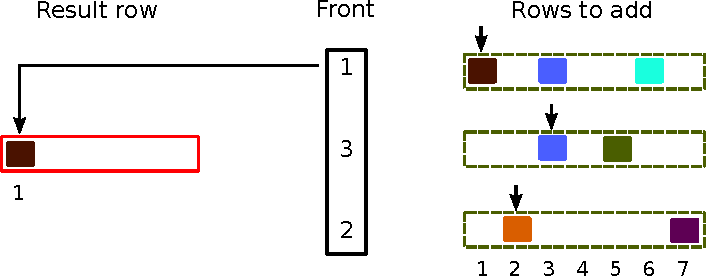
\includegraphics[width=0.85\textwidth]{row/spgemm-row-1}\\
a)\\
\vspace*{6mm}
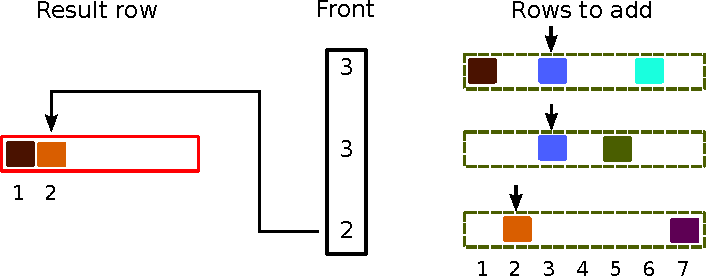
\includegraphics[width=0.85\textwidth]{row/spgemm-row-2}\\
b)\\
\vspace*{6mm}
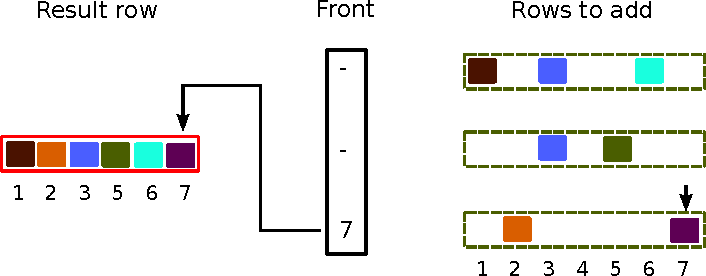
\includegraphics[width=0.85\textwidth]{row/spgemm-row-6}\\
c)\\
\vspace*{6mm}
\caption{Symbolic matrix-matrix multiplication with the \textit{rowmerge} algorithm. Figures by Karl Rupp \cite{karli_LANS_image}.}
\label{fig:spgemm-row}
\end{figure}


\subsection{Intel MatMatMult}
An implementation that was written in the course of this thesis is based on an idea by Patwary et al. of Intel \cite{intel_algorithm}. It is similar to the \textit{sorted} algorithm, so it also uses a dense array with a length of the number of columns in the matrix. The difference to the \textit{sorted} algorithm is that the  numerical calculation is performed at the same time as the symbolic calculation. This algorithm is sketched in Listing~\ref{alg:intel}.

The first step here is an iteration through all rows of $A$ (L5), where an upper bound on the memory requirements of $C$ is determined, which is followed by allocating memory for the matrix $C$ (L11). This includes memory for the arrays \texttt{ca}, \texttt{cj}, \texttt{cj} and for the dense arrays \texttt{c\_row\_val\_dense} (for the numerical values of a row of C) and for \texttt{c\_row\_idx\_flags} (for the flags that indicate if a specific column index has been added to the result).

Subsequently (L13), iterations over all rows of $A$ and, within that loop (in this row), iterations over all non-zero columns of $A$ are carried out. A third nested loop iterates through all non-zero columns of the current row in $B$. 

For the next step -- adding a column index to the array -- there are two different implementations: One implementation uses the \texttt{appendIndexToArray()} function (L29), the other one uses the \texttt{insertIndexInArray()} function (L34). For \texttt{appendIndexToArray()}, there is a dense bit array with index flags that indicate if a column index has already been added to the array. So if the corresponding flag is not set yet, an index can be added to the end of the array. The other option is to search the array for the index every time when the program passes this point, and add the index only if it is not present yet. Of course, \texttt{appendIndexToArray()} has a better computational complexity than \texttt{insertIndextoArray()} ($O(1)$ vs $O(n)$), but it also needs an additional array with a length that is the number of columns in $B$.

Independent of the choice of this function, the numerical value is updated (L40).

After the current row of $A$ has been processed, it is known how many non-zero indices\footnote{In the following, column indices that refer to non-zero entries are abbreviated to non-zero indices and analogously, non-zero columns for columns with non-zero entries.} there are in the current row, so the array \texttt{ci} can be updated (L45). Also, the array with the column indices has to be sorted (L44) and the numerical values have to be copied from the dense array to the result array \texttt{ca} (L51). Then the index flags can be unset (L54) and the dense numerical array (L57) can be reinitialized with zero, so that everything is ready for the next row of $A$.


After every row of the matrix $A$ has been processed like that, the sequential matrix can finally be created with the arrays \texttt{ca}, \texttt{ci}, and \texttt{cj} (L60).




\belowcaptionskip=-10pt
\lstinputlisting[label=alg:intel,caption={A pseudo-code sketch of the Intel algorithm for sequential sparse matrix-matrix multiplication. The symbolic and numeric values are calculated at the same time.}]{intel_seq.cpp}


\section{Numeric Phase}
The symbolic phase is followed by a numeric phase where the numerical values are finally calculated. All sequential implementations of the symbolic phase use the same algorithm for this numeric phase. Since there is no need to maintain an order of column indices in a data structure (as it is the case for the symbolic phase), this numeric phase entails much less work than the symbolic phase.

In the numeric phase, the steps of Fig.~\ref{fig:spgemm-numeric} are performed for each row of the result matrix \textit{C}: The rows of $B$ (with dashed green frame) have to be added to each other. The $j$-\textit{th} row of \textit{B} is assumed to be already scaled with the $j$-th entry of the $i$-th row of \textit{A} (\ref{fig:spgemm-numeric}a).

Now all rows that were first scaled with an entry of \textit{A} (that is as many rows as there are non-zeros in the current row of \textit{A}) have to be summed up into one single array. Here, a dense temporary row is used (\ref{fig:spgemm-numeric}b). 

After that, only the non-zero elements of this array are copied to the final current final result row of \textit{C} (Fig.~\ref{fig:spgemm-numeric}c). The indices of this row are already known because they were determined in the symbolic stage by one out of several possible algorithms.


\begin{figure}[H]
\centering
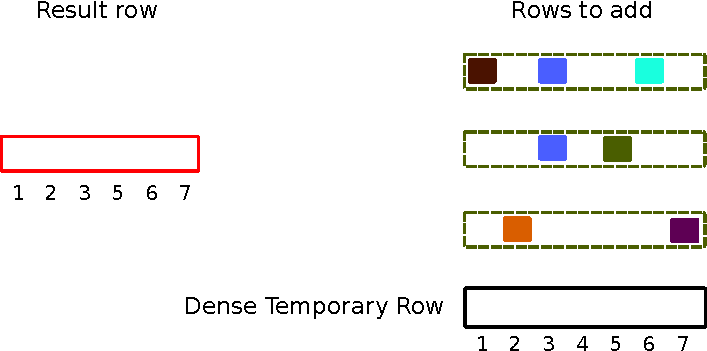
\includegraphics[width=0.72\textwidth]{spgemm-numeric-2}\\
a)\\
\vspace*{5mm}
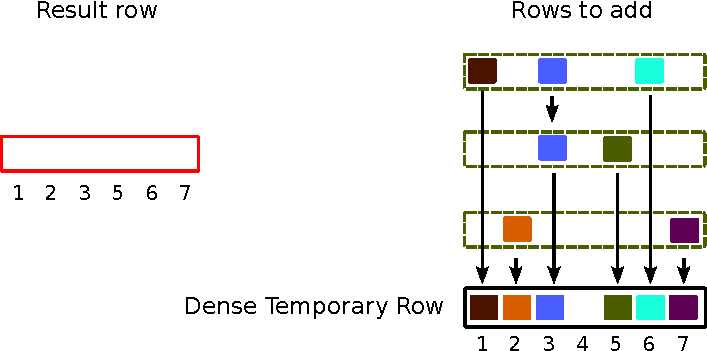
\includegraphics[width=0.72\textwidth]{spgemm-numeric-4}\\
b)\\
\vspace*{5mm}
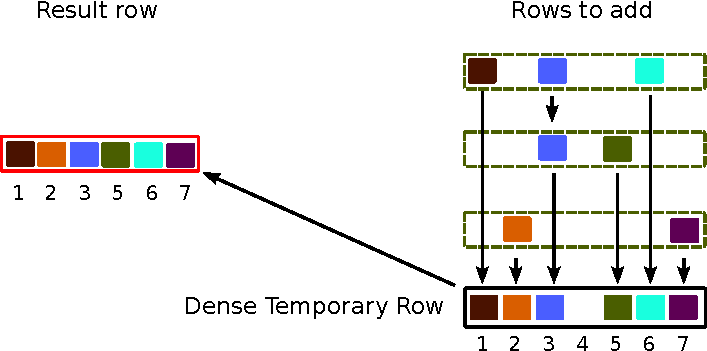
\includegraphics[width=0.72\textwidth]{spgemm-numeric-6}\\
c)\\
\vspace*{5mm}
\caption{Numeric sparse matrix-matrix calculation. Figures by Karl Rupp \cite{karli_LANS_image}.}
\label{fig:spgemm-numeric}
\end{figure}


\section{Parallelizing the Multiplication}

If several processes work at the same time on a matrix multiplication, they compute different rows of \textit{C}. A process that computes the row $c_i$ only needs the row $a_i$ of \textit{A}, but different rows of \textit{B}, and many of them might be local to other processes. That means a lot of data of \textit{B} has to be transferred over the network. Still, each process uses only local rows of $A$ for the matrix multiplication.

Fortunately, the non-zero entries of \textit{A} very often primarily lie on the diagonal of \textit{A}. Fig \ref{fig:matmult_diagonal} shows what this means: If the matrix \textit{A} only has entries on its diagonal portion, each process only uses local rows of \textit{B} for the computation. This is a very convenient property of matrix multiplication and one of the reasons why diagonal and off-diagonal entries are stored separately. That way, the diagonal parts can be computed while the rows $b_i$ that correspond to the off-diagonal parts of \textit{A} are being retrieved. As a consequence, stalls due to waiting for non-local elements are reduced. 

\begin{figure}[tb]
\centering
{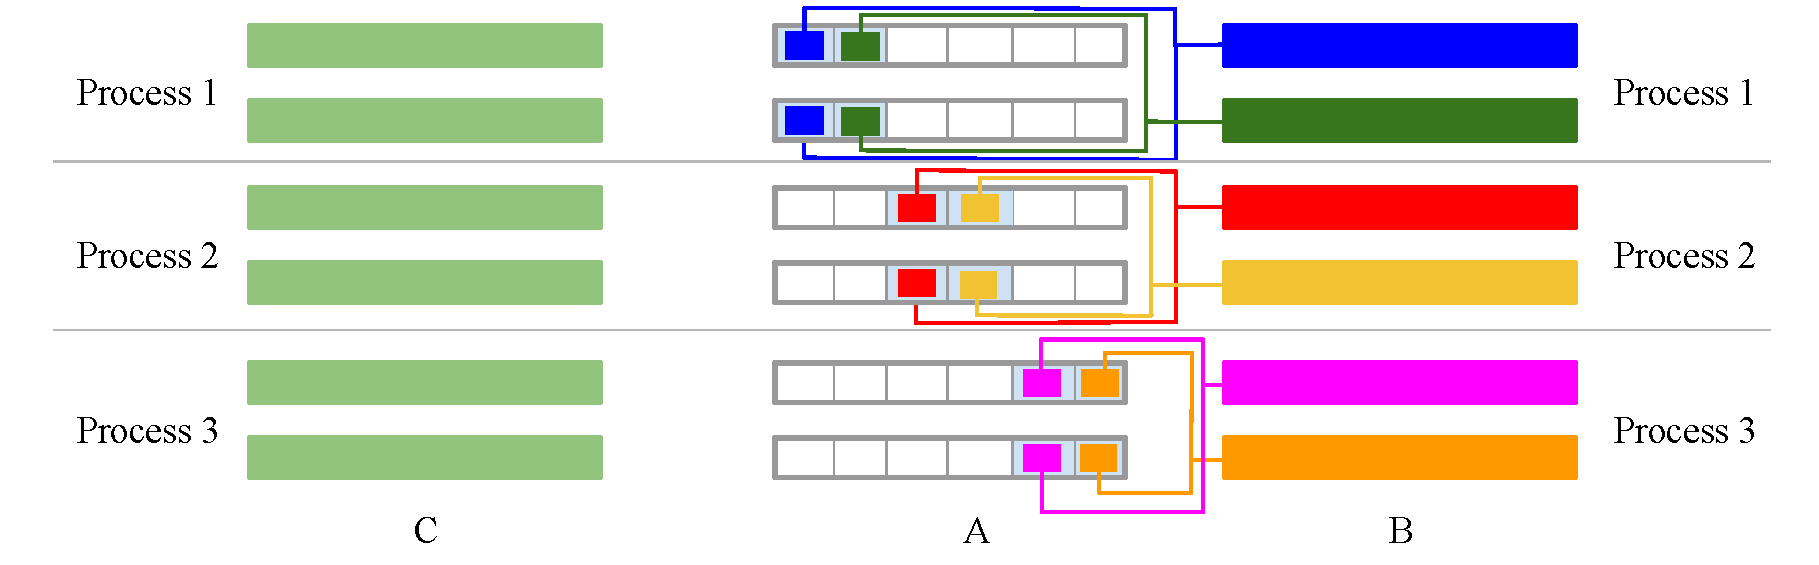
\includegraphics[width=1.05\textwidth]{matrix_multiplication_diagonal}}
\caption{Multiplication of two $6\times 6$ matrices with three processes: If the matrix \textit{A} has entries only in its diagonal part (highlighted in light blue), only local rows of \textit{B} have to be used.}
\label{fig:matmult_diagonal}
\end{figure}

On the other hand, if there are any off-diagonal elements in $A$, the process has to request non-local rows of $B$, as can be seen in Fig.~\ref{fig:parallel-2}. 


\begin{figure}[tb]
\centering
\vspace{5mm}
{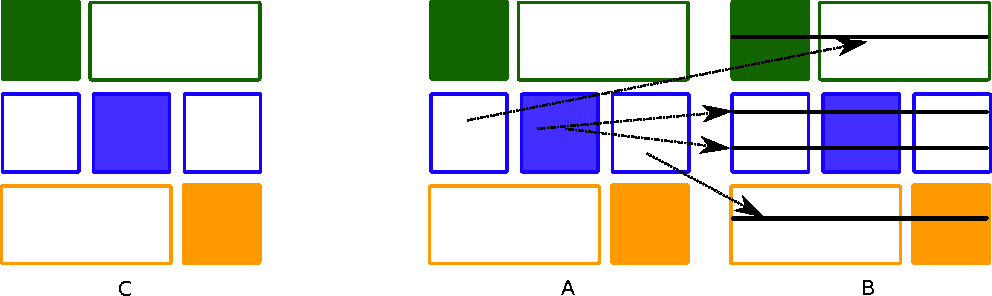
\includegraphics[width=0.95\textwidth]{parallel/spgemm-parallel-2} Figures by Karl Rupp \cite{karli_LANS_image}.}
\caption{If there are off-diagonal elements in $A$, the process has to retrieve rows of $B$ from other processes.}
\label{fig:parallel-2}
\end{figure}



Increasing the number of processes of course increases the raw computing power, but it also means that the width of the diagonal portion of \textit{A} decreases, which, in turn, means that more rows of \textit{B} are non-local and  more traffic between nodes is necessary. Therefore, it is possible that the performance decreases when the number of processes increases.

The parallel implementation in PETSc is again divided into a symbolic phase that is followed by a numeric phase. 


\section{Symbolic Phase of the Parallel Algorithm}
In PETSc, there are two existing implementations of the symbolic phase for the parallel matrix-matrix multiplication. Similar to the sequential case, these implementations are either scalable or not scalable and again, the difference lies in the memory requirements; the non-scalable implementation has a complexity of $O(N_B)$ (with $N_B$ being the number of columns in $B$), and the scalable implementation only needs $O(\textit{nnz}_B)$ memory (with \textit{nnz}$_B$ being the number of non-zeros in $B$).

\subsection{Existing Implementations of Parallel MatMatMult}
\label{sec:existing_impl}
The scalable and the non-scalable implementations of the symbolic parallel matrix matrix multiplication are almost the same. The only difference is that a fixed-size list is implemented for the non-scalable case (its length is the number of columns in the matrix $B$), while the list in the scalable implementation grows when more non-zero entries are found in the course of the multiplication. Due to these similarities, they are now both discussed at the same time.


Listing~\ref{alg:par_nonscalable} shows the most important steps of the symbolic phase of the scalable and non-scalable parallel matrix-matrix multiplication. The program starts with requesting the non-local rows of $B$ that correspond to non-zero indices of $A$ (L4). The next step is the actual matrix multiplication, which is performed by splitting the multiplication into two multiplications 
\begin{equation}
C_{\textrm{loc}} = A_{\textrm{loc~}} B = A_{\textrm{loc, diag~}} B_{\textrm{loc, diag}} + A_{\textrm{loc, off~}} B_{\mathrm{nonloc}}.
\end{equation}
One row of each product is calculated, then both rows are added (merged), before continuing to the next row. This works with nested iterations in the following way. 

The outer loop iterates over all local rows of $A$ (L7) and the inner loop iterates over all columns with non-zero entries in the diagonal portion of the current row of $A$ (L9). Now all indices of the row  of $B$ that corresponds to the current column of $A$ are copied to the sorted list (without creating duplicate entries, L13). 

After the diagonal entries of $A$ are fully processed, the same is done with the off-diagonal entries (L18). Subsequently, the entries in the \texttt{ci} array have to be updated (L27), i.e., another entry that gives information about the number of non-zero entries in the current result row has to be created (see Section~\ref{sec:csr_format} about the CSR format). 

Now that all information about the column indices for non-zero entries of one row has been computed,  it has to be copied from the sorted list to some other memory space, so that the memory for the sorted list can be used for the next iteration, i.e. for the next row of $A$ (L29). In the \texttt{setDnzOnz()} function that follows (L32), information on how many non-zero entries there are in the diagonal and off-diagonal parts of the current row is added to the \texttt{dnz} and \texttt{onz} arrays.

Next (L34), the list has to be reinitialized, so that it is ready for the next iteration (the next row of $A$). This list is the only difference between the scalable and the non-scalable implementation. While a scalable list might suffer from many slow memory reallocations, the non-scalable list needs much more memory.

When all local rows of $A$ (and therefore all local rows of $C$) have been processed, the results can be copied from the memory space to the result array \texttt{cj} (L37).

After that, the parallel matrix \texttt{Cmpi} can finally be created (L390). In order to get a high performance, it is crucial to preallocate each row of the matrix by using information from the arrays \textit{dnz} and \textit{onz} (L41). If this is done correctly, it is not necessary to allocate new memory and copy data from the old storage location to the new one, which is very expensive \cite{petsc-web-page}. Now the column indices are written to the matrix in a row per row manner, and a subsequent call to\texttt{MatAssembly()} (L46) finalizes the symbolic phase of the matrix multiplication.

\belowcaptionskip=-10pt
\lstinputlisting[label=alg:par_nonscalable,caption={A pseudo-code sketch of the existing algorithm for the symbolic part of the parallel sparse matrix-matrix multiplication.}]{parallel_non.cpp}


\subsection{A New Implementation of Parallel MatMatMult}
\label{sec:seq_mpi}
The just discussed scalable and non-scalable implementations first perform the calculation of one row of $C$ with the local part of $B$ ($A_{\textrm{loc, diag~}} B_{\textrm{loc, diag}}$), and subsequently with the non-local part of $B$ ($A_{\textrm{loc, off~}} B_{\textrm{non, loc}}$), before continuing to the next row of $C$, where the calculation with the local part is started again. This means that the non-local part of $B$ is needed very early in the computation, so the program has to wait until this non-local part is made available to the process.

A new approach is to first request the non-local part in the beginning of the program. Then the calculations that can be done with the local part of $B$ are performed while the non-local rows are still being retrieved. The matrix multiplication is then calculated as the sum of three matrix products 
\begin{equation}
C_{\textrm{loc}} = A_{\textrm{loc~}} B = A_{\textrm{loc, diag~}} B_{\textrm{loc, diag}} + A_{\textrm{loc, diag~}} B_{\textrm{loc, off}} + A_{\textrm{loc, off~}} B_{\textrm{nonloc}},
\end{equation}
where only the last product relies on non-local rows. This asynchronous flow is shown in Fig.~\ref{fig:mpi_workflow}.

\begin{figure}[tb]
\centering
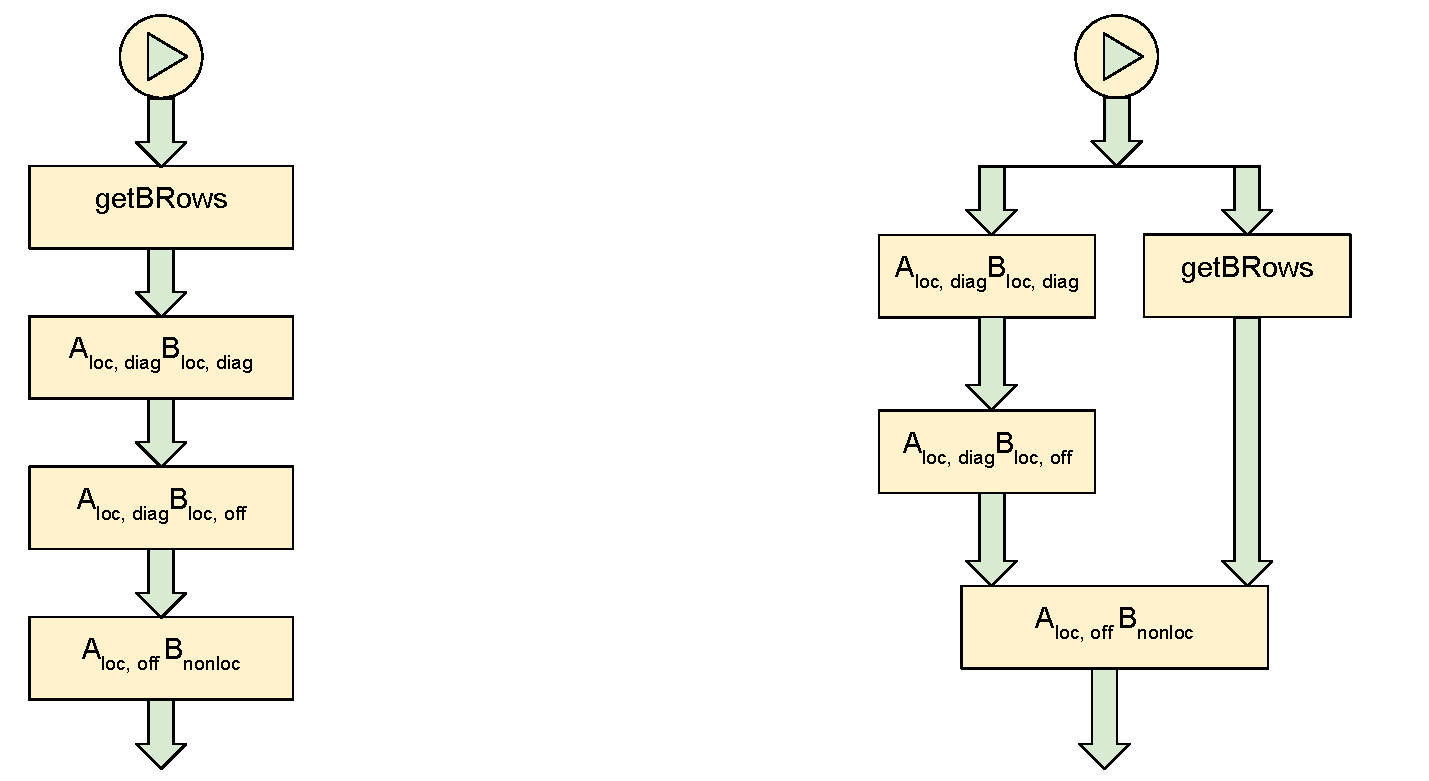
\includegraphics[width=0.95\textwidth]{mpi_workflow}
\caption{\textit{Left:} The work flow with as it is implemented in the new implementation: The matrix multiplication is split in three parts and non-local rows of \textit{B} are retrieved before any matrix calculations start. \textbf{Right:} The non-local rows of \textit{B} are retrieved at the same time as local multiplications are performed. This is not implemented yet.}
\label{fig:mpi_workflow}
\end{figure}

When calculating these products, the multiplications 
$A_{\textrm{loc, diag~}} B_{\textrm{loc, diag}}$ and $A_{\textrm{loc, off~}} B_{\textrm{nonloc}}$ can be fed to an existing, sequential implementation of the matrix multiplication. However, this is not possible for
$A_{\textrm{loc, diag~}} B_{\textrm{loc, off}}$. The reason for that is that the existing implementation of the sequential matrix multiplication always uses the local column indices of the input matrices. For $A_{\textrm{loc, diag~}} B_{\textrm{loc, off}}$ however, the local column indices of $A$ do not fit to the row indices of $B$. For the other two multiplications, the two factors can just be multiplied with each other because even with local indices, $a_{ij}$ still refers to a column $b_j$. After a simple transformation from the local index to a global index, the result of this product can be used.

In the course of this thesis, only the separation of the multiplication into three multiplications, of which two are carried out by existing procedures, was implemented. Changing the program to run in an asynchronous way, i.e. starting local calculations before non-local rows have arrived, can be implemented at a later stage. %However, as shown in the next chapter, only around 5\% time reduction can be gained from this approach. 
Since the new implementation provides a more ordered program execution, performance improvements can even be expected if it runs in an asynchronous way.



\subsubsection*{The algorithm}
The algorithm then works as shown in Listing~\ref{alg:new}. Like in the previous algorithm, the function starts with requesting the non-local rows of $B$ that will be used by that process. Then the first matrix product $A_{\textrm{loc, diag~}}B_{\textrm{loc, diag}}$ is computed by using the sequential version of the matrix multiplication algorithm (L6). 

Next, the product $A_{\textrm{loc, diag}} B_{\textrm{loc, off}}$ has to be computed. For that, iterations similar to the ones in previous algorithms are used (L8): The nested loops iterate through rows of $A$ in the most outer loop, and columns of $A$ in the next loop, then through columns of $B$. Since the column indices of the diagonal and the off-diagonal part always start with 0, no matter what the actual global index is, this index has to be corrected. This most inner loop does exactly that; here the column indices are transferred from a local to a global space. This is very simple because an array stores the global index of each entry.

After that, the row of $B$ is copied to a sorted list again (L15). In the outer loop, the result row is finished by updating the \textit{i}-array \texttt{ci} (L17), copying the list to a free space in memory (L19), and reinitializing the list (L21), just like in the \textit{non-scalable} and \textit{scalable} algorithm. When this outer loop is finished, all result indices are copied from the memory space to \texttt{a\_loc\_diag\_b\_loc\_off} (L27).

\begin{figure}[tbp]
\centering
\vspace{5mm}
{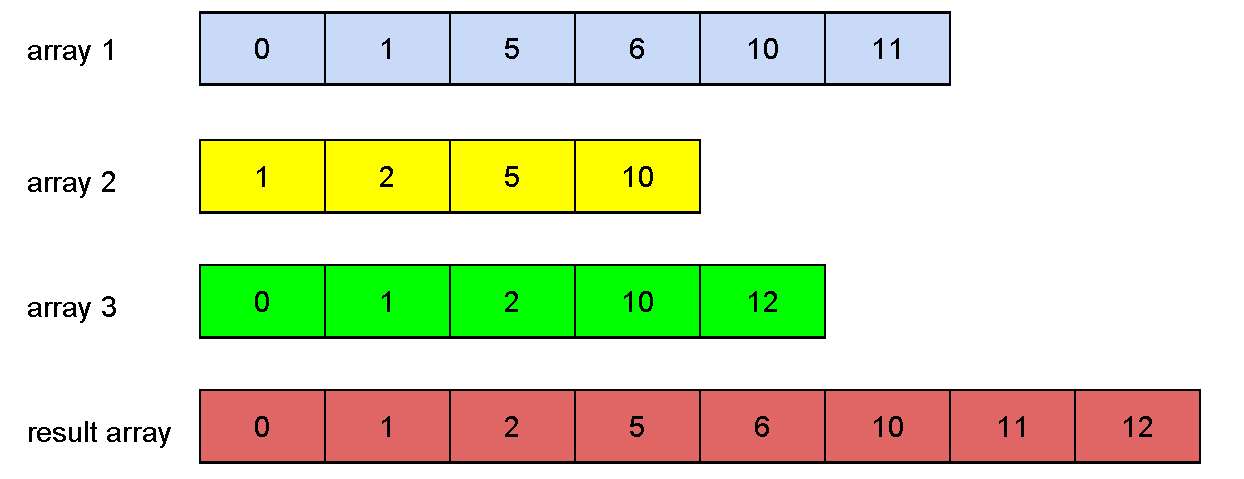
\includegraphics[width=0.9\textwidth]{mm_rowmerge}}
\caption{The three arrays with the column indices of the results of the multiplications $A_{\textit{loc,diag~}}B_{\textit{loc,diag}}$, $A_{\textit{loc,diag~}} B_{\textit{loc,off}}$ and $A_{\textit{loc,off}~} B_{\textrm{nonloc}}$ have to be merged.}
\label{fig:rowmerge}
\end{figure}

Now the calculation of $A_{\textit{loc, off}} B_{\textit{nonloc}}$ can start (L26). This is also implemented by executing an existing, sequential version of matrix multiplication. 

Next, the addition of these three matrix products starts (L27). That just means that the three arrays containing the j-indices are merged row by row, as can be seen in the example in Fig.~\ref{fig:rowmerge}. This is exactly the same principle as in the sequential \textit{rowmerge} algorithm. The only difference is that here result rows of three products are merged, while in \textit{rowmerge} many rows of \textit{B} are merged.


First however, the column indices of the product $A_{\textit{loc, diag}}B_{\textit{loc, diag}}$ have to be corrected, because the rows of this product always start with zero (L29). Therefore, the global row number of the first local row of the process has to be added to the column index, as illustrated in the example in Fig.\ref{fig:diag_row}. This results in the global column index.

\begin{figure}[tbp]
\centering
{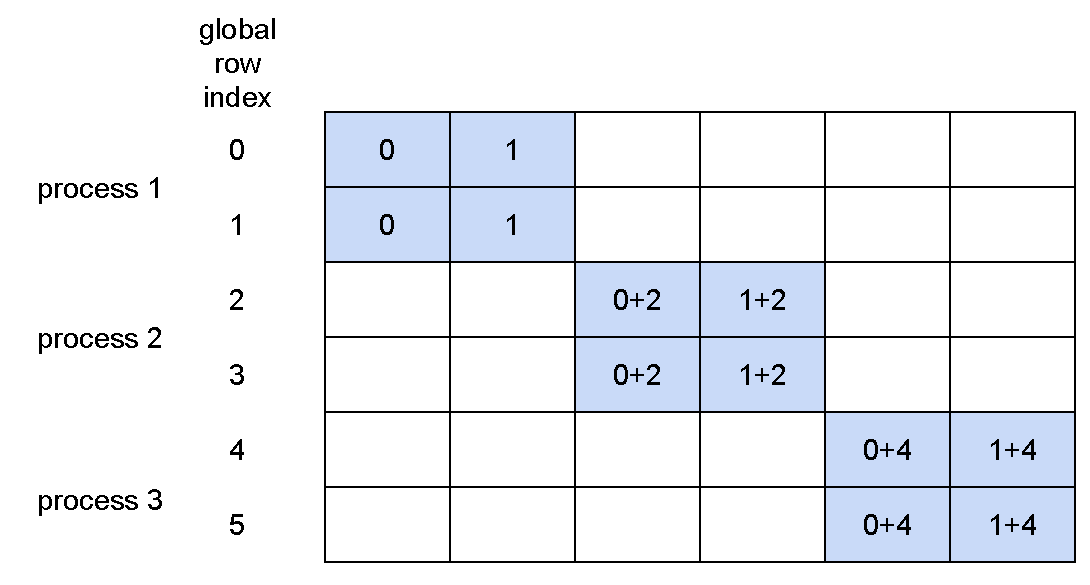
\includegraphics[width=0.7\textwidth]{mm_diag_row}}
\caption{A $6 \times 6$ matrix is divided between three processes. Since the column index in the diagonal part of the matrix always starts with 0, each process has to add the global row index of its first local row in order to obtain a global column index.}
\label{fig:diag_row}
\end{figure}

After each row has been merged to one result row of $C$, the arrays with information about non-zeros can be set again (L39) and  another \texttt{ci} entry is added (L40). When all rows of $C$ are finished, the parallel matrix \texttt{Cmpi} is again created by preallocating each row and then setting the entries for each row.
\vspace{5mm}

\belowcaptionskip=-10pt
\lstinputlisting[label=alg:new,caption={A pseudo-code sketch of the algorithm that uses sequential multiplications for parallel sparse matrix-matrix multiplication.}]{parallel_new.cpp}


\section{Numeric Phase of the Parallel Algorithm}

The symbolic phases of the three discussed parallel implementations of matrix multiplication are succeed by numeric phases that are almost the same for all implementations. 

This algorithm can be seen in Listing~\ref{alg:par_numeric}. After the non-local rows of $B$ are fetched (L5), there are iterations over all rows of $C$. The computation is again split into
\begin{equation}
C_{\textit{loc}} = A_{\textit{loc~}} B = A_{\textit{loc, diag~}}B_{\textit{loc}} + A_{\textit{loc, off~}}B_{\textit{nonloc}}
\end{equation}
 in such a way that first one row of the first product is calculated, then one row of the second product is added to that result.

\begin{figure}[tb]
\centering
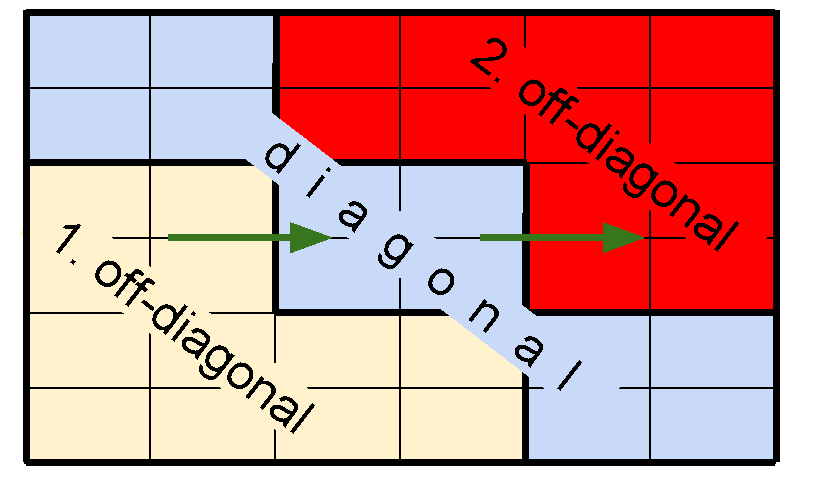
\includegraphics[width=0.65\textwidth]{mm_diag_offdiag}
\caption{Copying a result row of a $6\times 6$ matrix from \texttt{c\_sparse} to the diagonal and off-diagonal portions of the result matrix: First the elements of the first off-diagonal are copied, then the diagonal elements, and finally the elements of the second off-diagonal.}
\label{fig:diag_row}
\end{figure}

In order to calculate such a product, there is an iteration over all non-zero columns of the current row of $C$ (L7). If the current column index is also a non-zero in the current row of $B$, the product of the current entry of $A$ and the current entry of $B$ is added to a sparse array (L12). Each element of this sparse array is one of the non-zero numeric values of the current row of $C$. 

After these two multiplications, the result row \texttt{c\_sparse} has to be divided among the diagonal and the off-diagonal parts of $C$. This just means that first all elements of \texttt{c\_sparse} that precede the diagonal are copied to the off-diagonal part (L28), then the diagonal elements of \texttt{c\_sparse} are copied to the diagonal part of $C$ (L35) and finally the second off-diagonal part of $C$ is written (L41). 

After all rows have been processed like that, a call to the function \texttt{MatAssembly}() updates all numerical values of the result matrix (L48).



\belowcaptionskip=-10pt
\lstinputlisting[label=alg:par_numeric,caption={A pseudo-code sketch of the numeric step for parallel sparse matrix-matrix multiplication.}]{parallel_numeric.cpp}
